\documentclass{article}
\usepackage{graphicx}
\usepackage[utf8]{inputenc}
\usepackage{listings}
\usepackage{color}
\usepackage{xcolor}
\usepackage{textcomp}

\definecolor{solarized@base03}{HTML}{002B36}
\definecolor{solarized@base02}{HTML}{073642}
\definecolor{solarized@base01}{HTML}{586e75}
\definecolor{solarized@base00}{HTML}{657b83}
\definecolor{solarized@base0}{HTML}{839496}
\definecolor{solarized@base1}{HTML}{93a1a1}
\definecolor{solarized@base2}{HTML}{EEE8D5}
\definecolor{solarized@base3}{HTML}{FDF6E3}
\definecolor{solarized@yellow}{HTML}{B58900}
\definecolor{solarized@orange}{HTML}{CB4B16}
\definecolor{solarized@red}{HTML}{DC322F}
\definecolor{solarized@magenta}{HTML}{D33682}
\definecolor{solarized@violet}{HTML}{6C71C4}
\definecolor{solarized@blue}{HTML}{268BD2}
\definecolor{solarized@cyan}{HTML}{2AA198}
\definecolor{solarized@green}{HTML}{859900}

\lstset{
  language=Ruby,
  upquote=true,
  columns=fixed,
  tabsize=2,
  extendedchars=true,
  breaklines=true,
  frame=single,
  numbers=left,
  numbersep=5pt,
  rulesepcolor=\color{solarized@base03},
  numberstyle=\tiny\color{solarized@base01},
  basicstyle=\footnotesize\ttfamily,
  keywordstyle=\color{solarized@green},
  stringstyle=\color{solarized@cyan}\ttfamily,
  identifierstyle=\color{solarized@blue},
  commentstyle=\color{solarized@base01},
  emphstyle=\color{solarized@red}
}
\begin{document}

\title{Tarea 1}
\author{Angel Caceres Licona}

\maketitle


\section{1er ejercicio}
Redondear correctamente las siguientes cifras:

\begin{enumerate}
    \item 3.14159 a cuatro cifras significativas es 3.142
    \item 0.0003436 a tres cifras significativas es 0.000344
    \item 0.01254348459 a tres cifras significativas es 0.125 
    \item 0.01254348459 a siete cifras significativas es 0.01254348
    \item 0.01254348459 a una cifra significativa es 0.01
    \item 10.001 a una cifra significativa es 10
    \item 10.001 a tres cifras significativas es 10.001
    \item 10.001 a cinco cifras significativas es 10.001
    \item 3.1417 a las centesimas es 3.14
    \item 10,680 a miles es 11,000
    \item 1.258 a unidades es 1
    \item 1.258 a decimas es 1.3
    \item 1340.9 a decenas es 1340
\end{enumerate}

\section{2o ejercicio}

Dada la definición

\begin{equation}
    \frac{|p*-p|}{p}<5 \times 10^{-t}
\end{equation}

procedemos a susutituir y obtenemos lo siguiente:
\begin{equation}
    -5 \times 10^{-3} <\frac{|0.001238-0.001234|}{0.001234}< 5 \times 10^{-3}
\end{equation}
es decir
\begin{equation}
    -0.00617 \times 10^{-3} < 0.000004 < 0.00617 \times 10^{-3}
\end{equation}
lo cual es correcto. Para el segundo inciso tenemos que
\begin{equation}
    \frac{|0.00124-0.001234|}{0.001234}<n \times 10^{-t}
\end{equation}
es decir 
\begin{equation}
    0.00486 < 5 \times 10 ^{-3}
\end{equation}
por lo tanto tenemos 5 cifras significativas y 3 decimales correctos.

\section{Tarea}

\begin{lstlisting}
    public strictfp class Suma {

        public static void main(String[] args) {
        Double resultadod = 0.0;
        Float resultadof = 0.0f;       
            for(int i = 1; i < 5001; i++) {
                resultadof = resultadof + 1/(i*i); 
            }
            System.out.println("El resultado sumando de izquierda a derecha con precision sencilla es " + resultadof);
            System.out.println("\n");
            System.out.println("-------------------------------------------------");
            resultadof = 0.0f;
            for(int i = 5000; i > 0; i--) {
                resultadof = resultadof + 1/(i*i);
            }
            System.out.println("El resultado sumando de derecha a izquerda con precision sencilla es " + resultadof);
            System.out.println("\n");
            System.out.println("-------------------------------------------------");
    
    
            for(int i = 1; i < 5001; i++) {
                resultadod = resultadod + 1/(i*i);
            }
            System.out.println("El resultado sumando de izquierda a derecha con precision doble es " + resultadod);
            System.out.println("\n");
            System.out.println("-------------------------------------------------");
            resultadod = 0.0;
            for(int i = 5000; i > 0; i--) {
                resultadod = resultadod + 1/(i*i);
            }
            System.out.println("El resultado sumando de derecha a izquerda con precision doble es " + resultadod);
            System.out.println("\n");
            System.out.println("-------------------------------------------------");
    
        }    
            
    }
\end{lstlisting}
La salida del programa es la siguiente: 

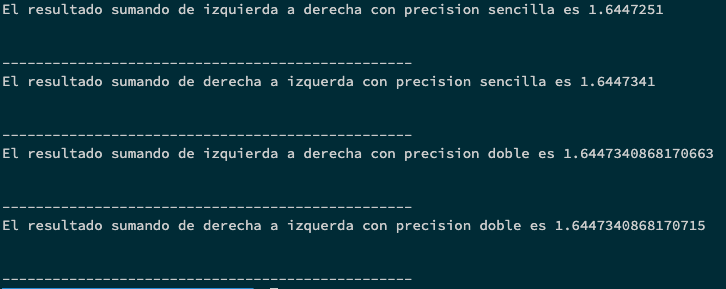
\includegraphics[scale=0.5]{SalidaJava.png}
por lo cual vemos que la precision doble sumando de izquerda a derecha es mejor.
\end{document}